%!TEX program = xelatex
% 完整编译方法 1 pdflatex -> bibtex -> pdflatex -> pdflatex
% 完整编译方法 2: xelatex -> bibtex -> xelatex -> xelatex
\documentclass[lang=cn,11pt]{elegantpaper}
% \usepackage{cite}

\title{State Machine}
\author{\href{https://github.com/Fassial/}{fassial}}

% \institute{\href{http://hyxt.whu.edu.cn/}{武汉大学 弘毅学堂}}

% 不需要版本信息,直接注释即可
% \version{0.07}
% 不需要时间信息的话,需要把 \today 删除。
\date{\today}

\def\BibTeX{{\rm B\kern-.05em{\sc i\kern-.025em b}\kern-.08em
		T\kern-.1667em\lower.7ex\hbox{E}\kern-.125emX}}
\begin{document}

\maketitle

\begin{abstract}
本文为Alveo-CiM项目内部所有状态机(state-machine)的介绍。
\keywords{Alveo-CiM, State Machine}
\end{abstract}

\section{声明}
\begin{enumerate}
	\item 本文档系Alveo-CiM项目\footnote{https://github.com/Fassial/Alveo-CiM}内部所有状态机的说明文档。
	\item 本文档只允许无修改原样分发,必须署名。
\end{enumerate}

\section{Tcam-Array}
\subsection{状态转移图}
Tcam-Array模块中的状态机所对应的状态转移图如图\ref{tcamArray}所示。
\begin{figure}[htbp]
	\centering
	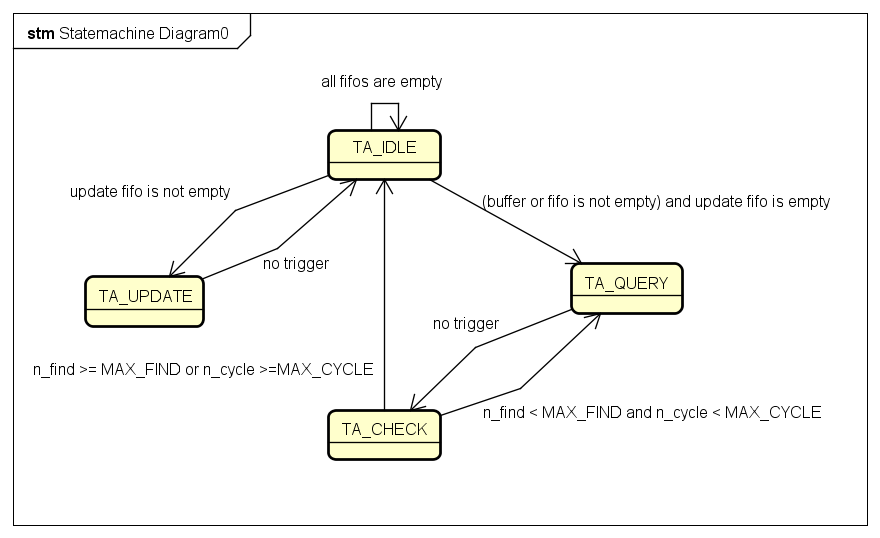
\includegraphics[width=0.8\textwidth]{tcamArray.png}
	\caption{Tcam-Array的状态转移图}
	\label{tcamArray}
\end{figure}
\subsection{状态转移解析}
Tcam-Array的状态有以下四种:
\begin{itemize}
	\item \textbf{TA\_IDLE}: 初始状态。状态机被重置时会被设定为该状态。该状态的转移情况如下:
	\begin{itemize}
		\item 在UPDATE\_FIFO、QUERY\_FIFO和FEEDBACK\_BUFFER全部为空的时候,会一直维持TA\_IDLE状态。
		\item 如果发现UPDATE\_FIFO不为空,说明有update请求,这时将会进入TA\_UPDATE状态,同时将update请求从UPDATE\_FIFO中取出,用寄存器进行锁存。
		\item 如果UPDATE\_FIFO为空,说明没有update请求,发现QUERY\_FIFO和FEEDBACK\_BUFFER(优先)不全为空,则进入TA\_QUERY状态,同时将所要查找的\{key, mask\}进行锁存。
	\end{itemize}
	\item \textbf{TA\_UPDATE}: 更新状态。该状态一般用于处理update请求。该状态的转移情况如下:
	\begin{itemize}
		\item 使用TA\_IDLE转移时记录的update请求对Tcam-Array内部的表项进行更新,一般只会耗费一周期,然后便转移到TA\_IDLE状态。
	\end{itemize}
	\item \textbf{TA\_QUERY}: 查询状态。该状态一般用于查询Tcam-Array。该状态的转移情况如下:
	\begin{itemize}
		\item 将TA\_IDLE或TA\_CHECK转移时记录的\{key, mask\}信息传入Tcam-Array进行查询,然后便进入TA\_CHECK状态。
	\end{itemize}
	\item \textbf{TA\_CHECK}: 检查状态。该状态一般用于检查Tcam-Array查询得来的结果。首先进行常规的更新,将n\_cycle累加,如果查到将n\_find累加并将index发往VALUE\_SRAM获得对应的value值放入scheduler,然后依据是否查到与Tcam-Array返回的index确定下一个\{key, mask\}组合。该状态的转移情况如下:
	\begin{itemize}
		\item 如果n\_find < MAX\_FIND且n\_cycle < MAX\_CYCLE,说明没有到达结束标准,转移至TA\_QUERY继续查询。
		\item 否则,说明查询结束返回TA\_IDLE。
	\end{itemize}
\end{itemize}
\textbf{注:如果scheduler接收到了来自后面流水的stall信号,会前传信号使得Tcam-Array内部的状态机不再更新状态。}

\section{NMC(Near-Memory-Computing)}
\subsection{状态转移图}
NMC模块中的状态机所对应的状态转移图如图\ref{NMC}所示。
\begin{figure}[htbp]
	\centering
	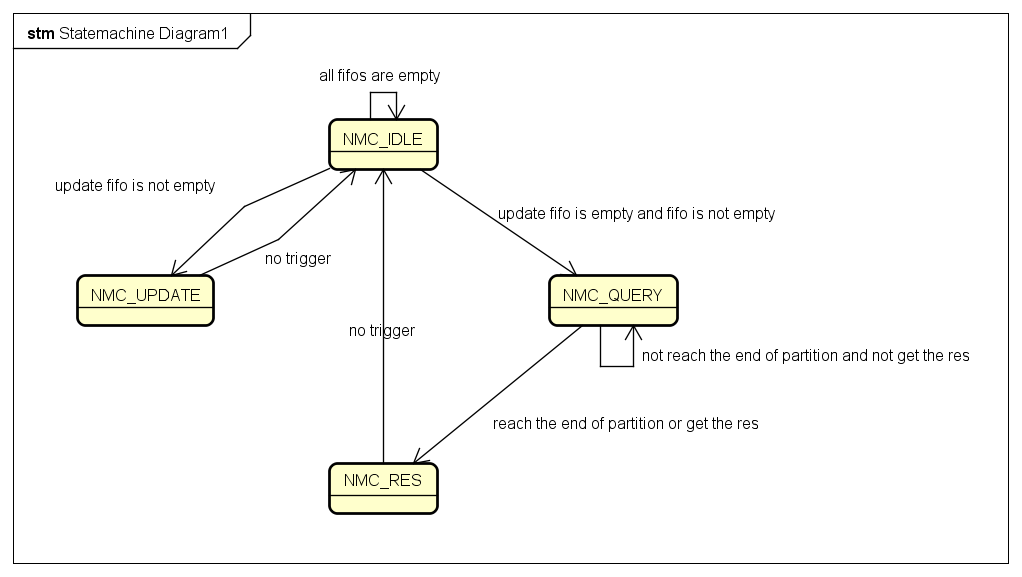
\includegraphics[width=0.8\textwidth]{NMC.png}
	\caption{NMC的状态转移图}
	\label{NMC}
\end{figure}
\subsection{状态转移解析}
NMC的状态有以下四种:
\begin{itemize}
	\item \textbf{NMC\_IDLE}: 初始状态。状态机被重置时会被设定为该状态。该状态的转移情况如下:
	\begin{itemize}
		\item 在UPDATE\_FIFO和QUERY\_FIFO全部为空的时候,会一直维持NMC\_IDLE状态。
		\item 如果发现UPDATE\_FIFO不为空,说明有update请求,这时将会进入NMC\_UPDATE状态,同时将update请求从UPDATE\_FIFO中取出,用寄存器进行锁存。
		\item 如果UPDATE\_FIFO为空,说明没有update请求,发现QUERY\_FIFO不为空,则进入NMC\_QUERY状态,同时将所要进行计算的feature和partition首地址进行锁存。
	\end{itemize}
	\item \textbf{NMC\_UPDATE}: 更新状态。该状态一般用于处理update请求(feature, res)。该状态的转移情况如下:
	\begin{itemize}
		\item 使用NMC\_IDLE转移时记录的update请求对NMC内部的表项进行更新,一般只会耗费一周期,然后便转移到NMC\_IDLE状态。
	\end{itemize}
	\item \textbf{NMC\_QUERY}: 查询状态。该状态一般用于查询NMC,并进行xnor运算。使用NMC\_IDLE转移时记录的feature信号和NMC\_QUERY自身记录的partitionId信息进行运算。该状态的转移情况如下:
	\begin{itemize}
		\item 如果到达了partition的底部(partitioonId不同)或者feature运算结果小于阈值,将进入NMC\_RES阶段,将结果寄存。
		\item 否则,说明没有找到结果且没有到达查询底部,维持NMC\_QUERY状态。
	\end{itemize}
	\item \textbf{NMC\_RES}: 结果阶段。这一阶段负责将NMC\_QUERY寄存的结果写入RES\_CACHE,结束本次partition查询。该状态的转移情况如下:
	\begin{itemize}
		\item 无触发,直接转移到NMC\_IDLE状态。
	\end{itemize}
\end{itemize}

\bibliographystyle{plain}
\bibliography{wpref}

\end{document}
